\documentclass[]{scrartcl}


\usepackage[english]{babel}
\usepackage{euscript}
\usepackage[utf8]{inputenc}
\usepackage[ruled,vlined]{algorithm2e}

\usepackage{graphics}

\usepackage[dvips]{graphicx}

\pagestyle{headings} \makeatletter

\usepackage{verbatim}


\usepackage{pictexwd,dcpic}


% quotient re-definition
\def\quotient#1#2{%
    \raise1ex\hbox{$#1$}\Big/\lower1ex\hbox{$#2$}%
}

% Margins
%\addtolength{\textwidth}{1cm}
%\addtolength{\marginparsep}{2cm}

\usepackage{makeidx}
\usepackage{eurosym}
\usepackage{amsfonts}
\usepackage{latexsym}
\usepackage{makeidx}
\usepackage{amsmath}
\usepackage{amsthm}
\usepackage{amscd}
\usepackage{comment}
\usepackage{enumerate}
\usepackage{mathrsfs}
\usepackage[all]{xy}

\DeclareMathOperator*{\argmax}{arg\,max}
\DeclareMathOperator*{\argmin}{arg\,min}

\usepackage{url}
\usepackage[colorlinks=true, a4paper=true, pdfstartview=FitV,
linkcolor=blue, citecolor=blue, urlcolor=blue]{hyperref}


\newtheorem{theorem}{Theorem}[section]
\newtheorem{corollary}{Corollary}[theorem]
\newtheorem{lemma}[theorem]{Lemma}

\theoremstyle{definition}
\newtheorem{definition}{Definition}[section]

%opening
\title{Bourbaki vs Pragmatism \\ A methodological comparison through the multi-armed bandits problem
 \\
 DRAFT
}
\author{Sebastiano Ferraris\footnote{sebastiano.ferraris@gmail.com}}

\begin{document}

\maketitle

% ------------------------------------------------- %
\begin{abstract}
    In these pages, through the example of the the multi-armed bandit problem, you will find a comparison between two methodological approaches to mathematics.
    The two methods are here named the \emph{Bourbachist} and \emph{pragmatic}: the Bourbachist way is concerned with the mathematical foundation upon which a formal solution emerges from a set-theoretical axiomatic structure. The other way, the pragmatic one, is focused on the algorithmic solution, and any underpinning mathematical formalisation appears only when needed.
    In this article you can also find a brief literature review about the history and origin of Bourbachism, and a shortlist of other notable examples where the same problem has been addressed in the Bourbachists' and in the pragmatic way. The article concludes with a final discussion about the advantages and disadvantages of each approach. \\

\noindent
If you discovered this article while searching for an introduction to the multi-armed bandit problem, please look directly at section~\ref{se:pragmatic_perspective}. The code to create the figures, to run and compare a range of solutions to the multi-armed bandit problem is version controlled and open to contributions at the link \href{https://github.com/SebastianoF/multi-armed-bandits-testbed}{https://github.com/SebastianoF/multi-armed-bandits-testbed}.
\end{abstract}


% ------------------------------------------------- %
\section{Two ways to approach the multi-armed bandits problem}
\label{se:intro}
Imagine you have to repeatedly choose between $K$ different options. All options have the same cost, though each may or may not provide you with a reward. The probability of having a reward is modelled by an \emph{unknown} distribution, that may be different for every option and that can vary over time.

This general setting is of concern for a wide range of problems, such as choosing a medical treatment or a drug, randomising quality control of produced parts, exploring new cafes, trying a range of cars before buying one, choosing a job, and for the most daring ones, selecting a partner. In the algorithmic literature the setting is referred to as the \emph{multi-armed bandits} (MAB), as it can be seen as the situation of playing repeatedly at a row of $K$ slot machines, and after the nickname \emph{armed bandit} for slot machines.

The reason why the algorithm takes its name form the gambling example and not from one of the others, more interesting and available in literature\footnote{
    For example Bouneffouf~\cite{bf2019survey}.
    }
is that the gambling case is the easiest to generalise and the one where the algorithmic machinery employed is also easier to visualise.
So, following the tradition, imagine to be on a trip to Las Vegas with an initial amount of money to invest in a row of $10$ slot machines. Let's say you start with $\$1000$, and that each draw costs $\$1$, this gives you $1000$ attempts to play and to balance an \emph{exploration} phase with an \emph{exploitation} phase. In the exploration phase the goal is to find an estimate for the unknown distributions of each arm. The exploitation phase aims at using the acquired knowledge to gain the highest possible reward in the face of uncertainty\footnote{
    Thompson~\cite{thompson1933likelihood} provides an early exposition to the method where the two arms are two medical treatments, Bellman~\cite{bellman1956problem} formulates the problem in a Bayesian perspective, again for two arms, and the more recent Sutton~\cite{sutton2018reinforcement}, Chapter~1, consider the problem as a starting point to introduce the field of reinforcement learning.
}.

The goal here is to provide a solution to the MAB problem, following two different mathematical approaches:
\begin{itemize}
    \item[$\circ$] \emph{Bourbachist approach.} Named after the collective pseudonym of the group of French mathematicians who have developed this viewpoint in 1934, it is driven by the need of providing a strict formalisation of the theory from a set theoretical perspective, whose conclusions are a consequence of a list of   axioms, and where the physical intuition is completely excluded.
    \item[$\circ$] \emph{Pragmatic approach.} In contrast to the Bourbachist approach, the pragmatic one reduces the formalisation to its bare minimum, and it orientates your efforts into finding a solution of a problem usable in practice, rather than creating a formal axiomatic theory.
\end{itemize}

Historically, the original goal of the Bourbaki group was to re-write one of the most widely used analysis textbook of the time, the Goursat’s \emph{Cours d'analyse mathématique}. This goal was motivated by the fact that the group found a few counterexamples contradicting some statements (Marmier~\cite{marmier2014idea}). To this end the Bourbachists ended up turning analysis into the pure manipulation of axiomatic systems, detached from any physical intuition, and the rewrote the whole corpus of mathematical analysis into a theory grounded on set theory and axiomatic systems, as generalisable as possible, and free from counterexamples. Subsequently the same approach had been then extended from analysis to other branches of mathematics, lead by the taste and desire for axiomatising and unifying all mathematics under the language of set theory. The feature that can be found in all books produced by Bourbaki any connection with the physical reality as well as the history motivating the given theorems are entirely omitted from the texts.

The MAB introduced in this section, is formalised \emph{à la Bourbaki} in the next one, and subsequently in the pragmatic way in section~\ref{se:pragmatic_perspective}.

% ------------------------------------------------- %

\section{The Bourbachist way}
\label{se:bourbaki_perspective}

\begin{definition}
    Let $(\Omega, \mathcal{A})$ be a $\sigma$-algebra defined as a non-empty set $\Omega$ paired with a subset of its power set $\mathcal{A}$, containing the empty set, and closed under numerable union and complement set. Let this be called an \emph{action space}. Let $\mathcal{I}_{K} = \{1,2, \dots , K\} \subset \mathbb{N}$ be a set of indexes whose generic element $k$ is called an \emph{arm}, by convention. Let $\mathcal{I}_{T} = \{1,2, \dots , T\} \subset \mathbb{N}$ be another set whose elements are called, again conventionally, \emph{time}. Let $\mathbb{R}_{+}$ be the positive real axis including the zero.
\end{definition}

The relationship between the above defined elements are given by an invertible function function $A$, defined as:
\begin{align*}
    A : \mathcal{I}_T \times \Omega &\longrightarrow \mathcal{I}_K \\
        (t, \omega) &\longmapsto A(t, \omega) = A_t(\omega)
\end{align*}
and by a function $\mathcal{R}$, defined as:
\begin{align*}
\mathcal{R} : \mathcal{I}_T \times \Omega &\longrightarrow \mathbb{R}_{+} \\
(t, \omega) &\longmapsto \mathcal{R}(t, \omega) = \mathcal{R}_t(\omega)
\end{align*}
Let the former be called \emph{action} and the latter be called \emph{reward}. 
We add to $A$ the property of $A_t^{-1}(\omega) \in \mathcal{A}$, for each $t \in \mathcal{I}$.
Let
\begin{align*}
R : \mathcal{I}_T \times \mathcal{I}_K &\longrightarrow \mathbb{R}_{+} \\
(t, \omega) &\longmapsto R(t, k) = R_t(k)
\end{align*}
be another function, based on which the function $\mathcal{R}$ becomes the composition  that makes the diagram below commutative, for each $t \in \mathcal{I}$:

\[
\begindc{\commdiag}[20]

% --- nodes:

% below
\obj(0,30)[R]{$ \mathbb{R}_{+} $}

% above
\obj(0,60)[Ik]{$ \mathcal{I}_K $}
\obj(-40,60)[A]{$ \mathcal{A} $}

% --- arrrows

% ortho
\mor{Ik}{R}{$R_{t}$}
\mor{A}{Ik}{$A_t$}

%  oblique
\mor{A}{R}{$\mathcal{R}_t$}

\enddc
\]
%
Let $R_t$ be called the \emph{reward's realisation}, or simply $\emph{reward}$ when there is no ambiguity.\\
We observe that $\mathcal{R}$ maps the elements $\Omega$, while $R$ maps the corresponding indexes, as their realisations. 

Now we consider
\begin{align*}
    \mathcal{Q} : \mathcal{I}_T \times \mathcal{A} &\longrightarrow \mathbb{R}_{+} \\
        (t, \omega) &\longmapsto \mathcal{Q}(t, \omega) = \mathcal{Q}_t(\omega)
\end{align*}
and we call it the \emph{estimated reward of the action $\omega$ up to time $t$}, for $\omega = A_t^{-1}(k)$ for a fixed $k\in \mathcal{I}_K$, with the corresponding function $Q: \mathcal{I}_T \times \mathcal{I}_K \rightarrow \mathbb{R}$. It follows that $\mathcal{Q}$ is defined as an application of the mean value in a Lebesgue space over $(\Omega, \mathcal{A})$, that is now a Borel $\sigma$-algebra\footnote{
    For a foundational perspective, see Bourbaki~\cite{bourbaki2004integration}.
} as:

\begin{align}\label{def:mathcalQt}
\mathcal{Q}_t(\omega) = \mathbb{E} \left[ R_{\tau}(k)\mid k = A_{\tau}(\omega)~~ \forall \tau \in \mathcal{I}_t \right]
\qquad
\omega \in \mathcal{A}
\qquad
t \in \mathcal{I}_T
\end{align}
and therefore its realisation
\begin{align}\label{def:Qt}
Q_t(k) = \mathbb{E} \left[ \mathcal{R}_{\tau}(\omega)\mid \omega = A_{\tau}^{-1}(k)~~ \forall \tau \in \mathcal{I}_t \right]
\qquad
t \in \mathcal{I}_T
\qquad
k \in \mathcal{I}_K
\end{align}
As $\mathcal{R}$ and $R$ did, also $\mathcal{Q}$ and $Q$ satisfies the commutativity of a diagram analogous to the one shown above. The notation can be simplified for brevity to:
% \footnote{
%     The simplified notation is often the only notation appearing in engineering textbooks (e.g. Sutton~\cite{sutton2018reinforcement}), although this would not allow you to understand the subtle formalisation of assigning to an event $\omega$ its index $k$. More tragically, if only the simplified notation is introduced, some may call that the concepts introduced before irrelevant and pedantic.
% } to:
\begin{align}\label{def:mathcalQt_simple}
Q_t(k) = \mathbb{E} \left[ R_{t}(k) \mid A_{t} = k \right]
\end{align}
where the mean value is for all the time indexes up to $t$ and where the domain values of $A_t$ is clear from the context. We remind the reader that the $k$ is constant to be constant for each $t\in\mathcal{I}_t$. We are now writing a definition that will be of use when we will be extending $k$ to be varying over $t$.

\begin{definition}
    Let the \emph{total reward} $Q_{\infty}: \mathcal{I}_K \rightarrow \mathbb{R}$ be the function
    \begin{align}\label{def:mathcalQinf}
    Q_{\infty}(k) = \mathbb{E} \left[ \mathcal{Q}_{t}(\omega) \mid \omega = A^{-1}_{t}(k)~~ \forall t \in \mathcal{I}_T \right]
    \qquad
    k \in \mathcal{I}_K
    \end{align}
    or with the simplified notation as:
    \begin{align}\label{def:mathcalQinf_simple}
    Q_{\infty}(k) = \mathbb{E} \left[ R_{t}(k) \mid A_{t} = k \right]
    \end{align}
\end{definition}

So far we have been considering the reward and the total reward for a fixed choice of $k$. We can vary $k\in \mathcal{I}_K$ in function of the time index. So let $\mathbf{k}$ be an element of
\begin{align*}
\mathcal{I}_K^T = \underbrace{\mathcal{I}_K\times \mathcal{I}_K \times \dots \times \mathcal{I}_K}_{T\text{-times}}
\end{align*}
or equivalently a function from $\mathcal{I}_T$ to $\mathcal{I}_K$.
Definitions \ref{def:mathcalQt} and \ref{def:mathcalQt_simple} are so generalised to $Q_t:\mathcal{I}_K^T \rightarrow \mathbb{R}$ for $t\in\mathcal{I}_{\leq T}$, having defined $\mathcal{I}_{\leq T}$ any interval of positive integers between~$1$ and $T$, and
\begin{align*}
Q_t(\mathbf{k}) = \mathbb{E} \left[ \mathcal{R}_{\tau}(\omega)
\mid
\omega = A^{-1}_{\tau}(\mathbf{k}_{\tau})~~ \forall \tau \in \mathcal{I}_t \right]
\qquad
\mathbf{k} \in \mathcal{I}_K^T
\qquad
t \in \mathcal{I}_T
\end{align*}
and therefore
\begin{align*}
Q_{\infty}(\mathbf{k}) = \mathbb{E} \left[ \mathcal{R}_{t}(\omega)
\mid
\omega = A^{-1}_{t}(\mathbf{k}_{t})~~ \forall t \in \mathcal{I}_T \right]
\qquad
\mathbf{k} \in \mathcal{I}_K^T
\end{align*}
The mean value computed with a Lebesgue measure, over the Borel space generated as the sets of images\footnote{
    We consider the definition under the accordance with the axiom of choice as in the ZFC axiomatic set theory, in order to avoid \emph{virages dangereux}. See also Bourbaki~\cite{bourbaki2004theory} and \cite{takeuti1982classes}.
} $\mathcal{R}_t(\omega)$ for all $\omega \in \mathcal{A}$ can be reformulated as:
\begin{align*}
Q_t(\mathbf{k})
=
\frac
{\sum_{\tau=1}^{t} R_{\tau}(\mathbf{k}_{\tau}) \mathbf{1}_{A_\tau = \mathbf{k}_{\tau}}}
{\sum_{\tau=1}^{t} \mathbf{1}_{A_\tau = \mathbf{k}_{\tau}}}
\end{align*}
where $\mathbf{1}_{A_\tau = \mathbf{k}_{\tau}}$ equals to $1$ for when the event $\omega$ corresponding to $\mathbf{k}_{\tau}$ is mapped exactly to $\mathbf{k}_{\tau}$ through $A_t$, and $0$ for any other event.
Extending the time indexes up to infinity, and to justify the notations introduced above, where we used $\infty$ for the finite case, we have the following theorem:
\begin{theorem}\label{th:bourbaki}
Given a ring of infinite cardinality to which the time index $t$ belongs, and an Hilbert module\footnote{An algebraic structure generalising Hilbert vector spaces over the now introduced ring of time indexes. See for example \cite{bourbaki1987topological}.} to which the vector $\mathbf{k}$ belongs, it follows that
\begin{align*}
Q_{\infty}(\mathbf{k}) = \lim_{T \rightarrow \infty} Q_{T}(\mathbf{k})
\end{align*}
\end{theorem}
\begin{proof}
    Direct consequence of the definition of $Q_{\infty}$. Details left to the reader.
\end{proof}

We now consider the value $\hat{k}$ that satisfies
\begin{align*}
\hat{k} = \argmax_{k \in \mathcal{I}_K} Q_t(k)
\qquad
\forall t \in \mathcal{I}_T
\end{align*}
for a constant value for each time index, as in the definition~\ref{def:Qt} of $Q_t$.
If you consider the possibility of varying the chosen arm $k$ across time, and so if you are allowed to compare different images of the function $A_t$, then $\hat{\mathbf{k}}$ is defined as
\begin{align}\label{eq:bourbaki_solution}
\hat{\mathbf{k}}
=
\argmax_{\mathbf{k} \in \mathcal{I}_K^{T}} Q_t(\mathbf{k})
\qquad
\forall t \in \mathcal{I}_T
\end{align}
Under the light of theorem~\ref{th:bourbaki}, and with the given definitions, we can now call the so defined vector $\hat{\mathbf{k}}$ the \emph{solution of the generalised multi-armed bandits problem}.

The attentive reader may have noticed a caveat. The realisation $R_t$ appearing in the first diagram, is defined upon a stochastic process, but it does not have the property of being random, in the sense that it is not define upon a sigma algebra. This abuse of notation to allow for a realisation is not the only possible option to re-build the whole axiomatic system.

To avoid this impasse that may cause contradictions in future developments based on the axiomatic structure given so far, we can instead define $R_t$ as the stochastic process:
\begin{align*}
    R_t : \Omega \times \mathcal{I}_K &\longrightarrow \mathbb{R}_{+} \\
    (\omega, k) &\longmapsto R_t(\omega, k)
\end{align*}

Now we define $\tilde{A}_t$ as the inverse of the projection of the first set $\pi_1 : \Omega \times \mathcal{I}_k \rightarrow \Omega$, $\tilde{A}_t = \pi_1^{-1}$, and $\mathcal{R}_t$
as the composition:

\[
\begindc{\commdiag}[20]

% --- nodes:

% above
\obj(-40,60)[Omega]{$ \Omega $}

% below
\obj(-40,30)[OmegaI]{$ \Omega \times \mathcal{I}_K $}
\obj(0,30)[R]{$ \mathbb{R}_{+} $}



% --- arrrows

% ortho
\mor{Omega}{OmegaI}{$\tilde{A}_t$}
\mor{OmegaI}{R}{$R_t$}

%  oblique
\mor{Omega}{R}{$\mathcal{R}_t$}

\enddc
\]
%

\noindent
As an exercise, the reader can reformulate the theorem~\ref{th:bourbaki} starting from the new definition of $R_t$ given above.


% ------------------------------------------------- %
\section{The Pragmatic way}
\label{se:pragmatic_perspective}

The first reasonable thing to do is to create a playground or a benchmark, where a ground truth of the multi-armed bandit problem is known. With this tool, where to test a range of algorithms and parameters, we can select a dataset and test a range of algorithms and ideas.

\subsection*{Creating a Benchmark}

We introduce the tool in a particular case, assuming each arm normally distributed, with mean sampled from a uniform distributions in the interval $[-3, 3]$ and the standard deviation sampled from a uniform distribution on the interval $[2, 3]$. A representation of these distribution is plotted in
figure~\ref{fig:volin_plot}.

If the studied case is modelled with a different distribution, what is said in this section is still applicable simply adapting this benchmark to the intended situation.

\begin{figure}[h]
    \hspace{-1.5cm}
    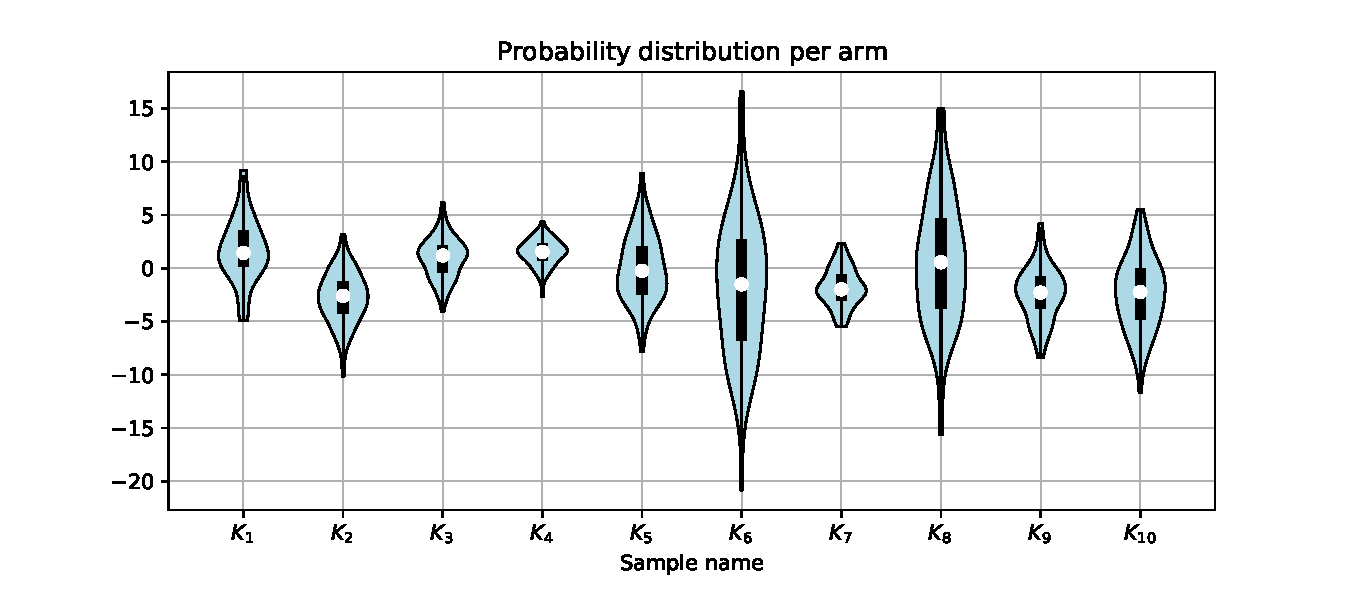
\includegraphics[width=18cm]{figures/initial_distributions.pdf}
    \caption{The distributions of the random reward for each arm $K$, unknown to the player, are sampled from normal distributions, with mean uniformly sampled in the interval $[-3, 3]$ and standard deviation in the interval $[1, 2]$.}
    \label{fig:volin_plot}
\end{figure}

\subsection*{Encoding the problem}
The player gains a reward for after pulling an arm index $k$, for each time point $t$. We encode the rewards in a $T\times K$ \emph{reward matrix} $q$. In our example $T=1000$ is the time we will be pulling an arm and $K=10$ is the number of arms. The element $q_{t, k}$ represents the reward collected for having pulled the arm $k$ at the time-point $t$. As we can pull only one arm at a time, there is only one known value for each column of the matrix. All the other values are initialised to nan.

The multi-armed bandit is defined by two vectors $\mu$ and $\sigma$, where $\mu_k$ is the mean and $\sigma_k$ is the standard deviation of the distribution of the arm $k$.
To consider the non-stationary case, where the means and the standard deviations of the arms distributions represented in Figure~\ref{fig:volin_plot} are not constant over time, we turns the vectors $\mu$ and $\sigma$ into matrices of size $T_{\text{arm}} \times K$, providing the mean and standard deviation of the distribution of the arm $k$ at time $t$.

The rewards can be accumulated for more or less numerous time points than $T_{\text{arm}}$, as the distributions of the arms can repeat. If $T_{\text{arm}}=1$ then the problem is stationary, and if $T=30$ and $T_{\text{arm}}=15$ then each arm $k$ will be looping over its parameters $\mu_{:, k}$ and $\sigma_{:, k}$ twice, according to:
\begin{align*}
q_{t, k}
=
\text{norm}\left(\mu({t~\text{mod}~T_{\text{arm}}, k}), \sigma({t~\text{mod}~T_{\text{arm}}, k})\right)
\end{align*}
where $\text{norm}(\mu, \sigma)$ is the normal distribution of location $\mu$ and scale $\sigma$ and mod is the modulo operator.

\subsection*{$\epsilon$-greedy algorithms}

In the previous section we created a benchmark and encoded the multi armed bandit response/rewards into a matrix.

Now we introduce the $\epsilon$-greedy algorithms,
a class of algorithms based on the idea that if your bad luck is consistent, probably it is not just bad luck. The player using these algorithms alternates between a phase of exploration (proportional to $\epsilon$ times), and a phase of exploitation (proportional to $1 - \epsilon$ times). In the first phase, the player acquires information about the structure of the problem regardless the immediate gain, and in the second one, the information gained are exploited to maximize the reward\footnote{
    An accurate historical introduction of this family of algorithms can be found at the end of chapter~1 of~\cite{sutton2018reinforcement}.
}.

The basic version of the $\epsilon$-greedy algorithm (or \emph{naive $\epsilon$-greedy}), selects a random arm when exploring and the arm that had obtained the best reward so far in the exploitation phase. This can happen after an initial phase of pure exploration, where only random arms are pulled. An example of the application of this algorithm is shown in figure~\ref{fig:step_32}.

A more sophisticated version the naive $\epsilon$-greedy is the \emph{best reward $\epsilon$-greedy}. In this case, instead of selecting any random arm in the exploration phase, we weight the random selection using the rewards obtained so far, excluding the arm with the highest reward. With this strategy we will be more likely to explore the arms that have provided good rewards in the past, and to refrain from spending money over an arm that have never provided any gain at all.

A third algorithm is the \emph{least explored $\epsilon$-greedy}. In the exploratory phase of this algorithm we increase the probability of falling over the least explored arms, instead of the one providing the highest reward. This method and the previous one are both aimed at preventing from getting stuck in a local minima, i.e. believing that the arm we are hitting is the best one, as it happens to provide a gain, though it is not the one with the optimal gain.

\begin{figure}[h]
    \hspace{-1cm}
    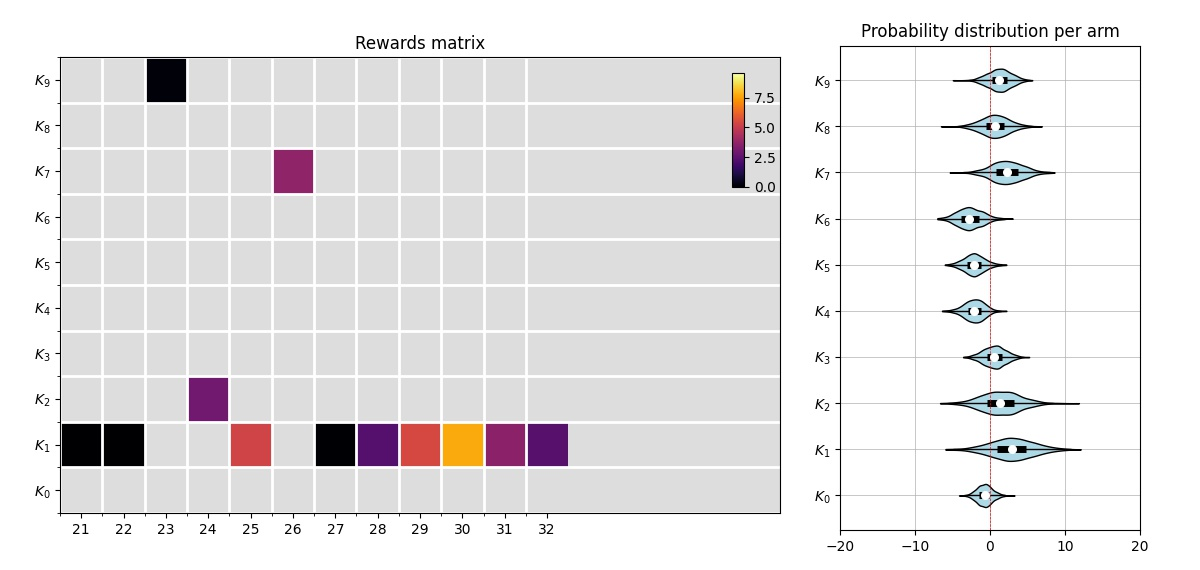
\includegraphics[width=17cm]{figures/step_32.jpg}
    \caption{The reward matrix after $32$ steps of a \emph{naive} $\epsilon$-greedy algorithm. We can see that step $23$, $24$ and $26$ are explorations in a row of exploitation of the arm $7$ that so far had produced the highest reward. To the grey colour corresponds the nan value used to initialise the reward matrix. In this instance, the reward is clipped at zero, as the loss of money is only the cost of pulling an arm at each time-point.}
    \label{fig:step_32}
\end{figure}

The fourth algorithm here presented is the \emph{upper confidence bound $\epsilon$-greedy algorithm} \cite{sutton2018reinforcement}. In this algorithm the estimated optimal arm at time $t$, is given by
\begin{align}\label{eq:upper_confidence_formula}
\hat{k}_t = \argmax_{k} \left[ \hat{\mu}(k) + \lambda \sqrt{ \frac{\ln(t)}{ N_{t}(k) }  } ~\right]
\end{align}
where $N_{t}(k)$ is the number of times the armed $k$ had been pulled up to the time $t$, which can be easily computed from $q$. The regularisation term weights the uncertainty in the estimate, correcting for underestimation of the estimated mean.

Note that in this version of the game, the player will receive $0$ when the sampled reward is below $0$. This means that the estimated mean does not correspond to the one of the original distribution, though the result will be conservative in having an observed average close to zero for distribution whose mean is below the zero. You should resist the temptation of estimating the arm using the mode instead of the average in equation~\ref{eq:upper_confidence_formula}. In fact if the standard deviations are very different across arms, a very inconvenient arm, with the average below the zero, may be identified as the optimal one.

The performance of these algorithms are all depending upon the problem's distributions, and the optimal one should be found empirically via simulation. Providing a benchmarking for a general case would not be useful here. What provides the constraints to make the case less general, is based on the instance of the problem to which the algorithms are applied. A platform where to make further experiments is open-sourced and can be found at~\href{https://github.com/SebastianoF/multi-armed-bandits-testbed}{https://github.com/SebastianoF/multi-armed-bandits-testbed}.


% ------------------------------------------------- %
\section{Comparing the two ways}
\label{se:outro}

The Bourbaki way presented in section~\ref{se:bourbaki_perspective} is based on an axiomatisation of the problem and it evolves from a functional and set-theoretical perspective. It focuses on the symbolism, and according to the Bourbachist tradition, it provides no examples or algorithms, as the only connecting point between the theory and the given problem is the axiomatic setting.

Assuming that section~\ref{se:bourbaki_perspective} is correct (excluding typos) and coherent (excluding Goedel\footnote{
    In the article \emph{The ignorance of Bourbaki}~\cite{mathias1992ignorance} Mathias noticed that the Bourbaki attempt of grounding the whole corpus of mathematics in an axiomatic sense have happened after, and with a conscious effort to ignore the Goedel incompleteness theorems.
}), it is easy to see that it had the side effect of turning a relatively simple problem into a complicated maze of interrelated concepts, whilst also pushing you away from the practical solution, and perhaps even entirely from mathematics.

On the contrary, the pragmatic approach of section~\ref{se:pragmatic_perspective} shows that there is no need to take a functional perspective, when a single matrix is enough. It shows that Borel spaces and Lebsgue Measures are not an important requirement. These tools have been developed in entirely different contexts to prevent counterexamples. There is also no need to extend the bibliography beyond one or two resources. Borel spaces and any element of measure theory are not just useless when aiming at a solution, they are also hindering creativity when facing a slightly different problem, as for example one with different types of distributions over time, or one where not all the arms are available at any point in time.

If you are in any doubt about this hindrance, you are invited to continue the formalisation started in section~\ref{se:bourbaki_perspective}, to see how many pages and new definitions and diagrams are needed to formalise the case of arms whose distribution varies over time. You are also invited to implement the algorithm solving the problem having only the functional and algebraic definitions at hand rather than relying on the matrix point of view.

%None of the given definitions in the Bourbaki approach had provided any hints on how to really solve the problem, in a numerical sense, as, in conformity with the Bourbaki style, no examples had been provided.

%https://www.synonyms.com/synonym/overzealous
%https://www.bbc.co.uk/worldservice/learningenglish/language/askaboutenglish/2009/03/090324_aae_hand_page.shtml

\subsection*{Other examples}

Certainly the example provided is biased by the fact that it consists of the best approximation of a Bourbaki approach and of a pragmatic approach that I could attain. Also you may say, the MAB problem is not the ideal one to embed into the Bourbaki formalisation, as \emph{per se} too empirical.

To answer these valid points, I wish to point out that the Bourbaki group intended to formalise the whole corpus of mathematics and that there are numerous cases of practical problems, whose pragmatic approach has been overly formalised\footnote{
    Or \emph{assiomattisation}, as Bruno de Finetti~\cite{de2008bruno} would have said playing on the Italian words \emph{assiomi} and \emph{matti}, crazy.
} as the one proposed here. These examples may also constitute a collection of case-studies for anyone who may believe that I  had been over zealous in writing section~\ref{se:bourbaki_perspective} to cast a negative light upon the Bourbaki methodology.

The first most notable example belongs to the domain of optimal transport theory. From being a pragmatic tool of solve a class of optimisation problems, it had become, in the hand of Bourbachists, a $500$ page book underpinned by a large amount of measure theory and Lebesgue spaces, perfectly irrelevant to solve any instance of an optimal transport problem. Comparing for example Hitchcock~\cite{hitchcock1941distribution} introduction to the formalised counterpart, written by Villani~\cite{villani2003topics} it is possible to see the Bourbachisations effects. The first work is easy to read, understand, implement and possibly extend in several directions by anyone having a high school mathematical education. The second one is a seemingly uncreated maze of unassailable interlinked concepts, requiring many years of academic studies only to grasp the first few pages, with no advantages in finding a numerical solution to the problem. %It is almost impossible to be extended in any direction that a slightly different initial problem arising from practical need may pose, and it leaves no clarification whatsoever about why this perspective should be preferred upon the one proposed 60 years before. %Not surprisingly, a recent evolution of the OT by Patel~\cite{patelalternate} is rooted in the pragmatic approach, and does not even cite the Villani formalisation.

The second example of the Bourbachisation that I found is in the domain of medical image registration. The aim of this field is to solve the problem of finding the non-rigid deformation, or metamorphosis, between anatomies. The problem originates from the study of the growth and change of anatomical shapes by D'Arcy Thompson~\cite{d1942growth} and pragmatically extended, amongst others, by Modersitzki~\cite{modersitzki2004numerical}. The Bourbaki over-formalized branch can be found in works such as Younes~\cite{younes2010shapes}, where we have to wait for 12 chapters before seeing what had motivated the axiomatic mathematical theory developed up until that point.
In this case too, there is no explanation of what the advantages of the axiomatic approach are in respect to the pragmatic one, which appeared half a century earlier.

You may now say, for this specific case, that the pragmatic approach \cite{modersitzki2004numerical} does not use neither diffeomorphisms nor reproducing Kernel Hilbert spaces. While this is true, it is not proved that these two mathematical devices are resulting in anything more accurate than their pragmatic counterparts when implemented in practice. Instead it is true that they are computationally slower and that they increase the cognitive load.


\subsection*{The Bourbaki standards}

There are other examples in the literature where it is possible to find a comparison between the Bourbachist / pragmatic way, such as with algebraic topology, fuzzy logic and topological data analysis. 
These branches of mathematics had been drawn out by Bourbachists from the practical set of solutions to problems into convoluted axiomatic constructions. Using their resource it is not possible to find any help in solving the problem initially given.

It is at this point evident the existence of a standardised pattern in the process of Bourbachisation: a problem solved by more than 50 years, and often in a very elegant and straightforward way, is taken under the wing of the academic axiomatisers and transformed into a list of definitions and theorems where no trace of the original problem motivating the theory can be found.

%Remarkably, also Einstein had noted that \emph{Since the mathematicians have invaded the theory of relativity, I do not understand it myself any more} \cite{schilpp1951albert}. And it is difficult to find what are the new results that the Bourbaki formalisation have added to the theory of relativity.

What is also a feature of the Bourbaki pattern is that the formalised version of the practical theory adds no value whatsoever. No new results having any practical relevance or impact can be found in the work by Bourbaki and their followers.

There is only one notable exception to this rule. The work by Mochizuki~\cite{mochizuki2012inter} is claimed to have solved the \emph{abc conjecture}. Although, worthy of pantomime, according to the mathematicians who had tried to read this work, \lq\lq the proof is too impenetrable to be understood\rq\rq\footnote{A statement published in Nature, Castelvecchi~\cite{castelvecchi2015biggest}.}.

\section*{The bright side of Bourbaki}

%What the examples proposed in these pages intended to show, from a qualitative and empirical evaluation, is that the over-axiomatic version of a theory has several negative aspects respect to its pragmatic counterpart.

%These are: Bourbaki formalisation has an exhaustive cognitive load,increases the difficulties that a generalisation of a simple change in the initial problem setting may require. It is by no mean close to the formalisation that is required to be implemented in modern programming language. Bourbaki does not provide any additional insight and intuition over the problem that originated the theory. You get used to work on useless details and pedantic discussions about notations, rather than solving the problem.


I am not here to criticize Bourbaki. The evil that men do lives after them. I am writing these pages to try to analyse and understand the phenomenon beyond its name and its influence.
It is true that, despite many have express their negative view about the Bourbachist's mathematics\footnote{
    Amongst the many: Arnold~\cite{arnol1998teaching}, De Finetti~\cite{de2008bruno}, Lockhart~\cite{lockhart2009mathematician}, the already cited Mathias and its follow up~\cite{mathias1998further}, Velupillai~\cite{velupillai2012bourbaki}. And even the article by Marmier~\cite{marmier2014idea}, that sees the Bourbaki movement with enthusiasm and appreciation for their work and impact in the society, begs some questions when it says
    \lq\lq Living mathematics is being done elsewhere in the world, in connection with new problems arising from other disciplines or other human activities\rq\rq.
}, the Bourbaki approach is still widespread if not predominant across the academic community and also greatly valued and honoured\footnote{
    To this regard, anyone is welcome to copy-paste section~\ref{se:bourbaki_perspective} and to extend it, in the Bourbachist style, into an article whose title could be something like \emph{The multi-armed bandits for the working mathematician}, to see how this would be received by the community.
}.

Very often, the over-axiomatisation of a theory developed outside academia by scientists chasing solutions to practical problems, had received more recognition than the original work.
Highly valued and cited uber-bourbachists works are for example Grotedniek~\cite{grothendieck2011some} and the aforementioned four impenetrable volumes by Mochizuki~\cite{mochizuki2012inter}\footnote{
    It is also interesting to notice at this point the similarity between this work and the outcome of the randomized generator of maths paper at \href{https://thatsmathematics.com/mathgen/}{thatsmathematics.com/mathgen/}.
}.

For this reason, it is not true to claim that the Bourbachisation has no practical use. Listed below are some points in favour of this approach, that are aimed at explaining its success.

\begin{itemize}
    \item[$\circ$] \emph{The outcome of the Bourbaki approach is inaccessible to novices}\footnote{
        An attempt of turning an over-formalised Bourbachist theory into something accessible for the layman, can be found in Villani~\cite{villani2003livingtheorem}. Interestingly enough, it seems that the only way the author could popularize his theory was to throw some unexplained formulas right before focusing the reader's attention on some entirely unrelated autobiographical events. The result is even less accessible than the original work, proving that mathematicians can also be successful surrealist artists.
    }, and it allows the existence of professors of mathematics who can neither code nor have experience in solving problems in practice.

    \item[$\circ$] \emph{The Bourbaki approach is good for the ego}. The pleasure of owning an elegant notebook filled with mathematical formulae written with a sharp pencil and on elaborate handwriting is a most sublime one. Unfortunately, this very same pleasure can become an obstacle in acquiring knowledge due to the tendency of bending the problem in favour of the beheld solution.

    \item[$\circ$] \emph{Bourbachism detaches mathematics from reality}, so it makes impossible to have any objective measurement of the quality or value of the work produced, besides the readers' opinion.

    The advocates of the superiority of \emph{pure mathematics}\footnote{
        And with another footnote, I would like to notice that the academic dichotomy pure/applied maths is something that can not be found in mathematics before Bourbaki. You are invited to classify any of the work by Archimedes, Gauss, Euler, Lambert, Poincare or any other great name at any time in the history of pre-modern mathematics as \emph{pure} or \emph{applied} with no ambiguities. It is also worth mentioning that there are few French mathematicians, contemporary of Bourbaki, that had been labelled as \emph{applied}, as Jean Leray, René Thom, Szolem Mandelbrojt (the uncle of Benoit Mandelbrot) for having left the group very early or for not having entered at all \cite{barcellos1984interview, atiyah2007bourbaki}.
    } have even arrived at accusing the mathematicians dealing with reality rather than abstract ideas of being more prone to make mistakes\footnote{
        Gros~\cite{gros2019masters} had found how even professional mathematicians can be mislead by reality. And they had leveraged on this most surprising fact, for advocating to increase the detachment. After concluding that \lq\lq [...] we can't reason in a totally abstract manner\rq\rq, instead of suggesting to take into account the reality in the mathematical practice they suggested a move towards the opposite direction: \lq\lq We have to detach ourselves from our non-mathematical intuition\rq\rq~\cite{gros2019sciencedaily}.
    }. It would be interesting to know what the authors of~\cite{gros2019masters} would think about detatching medicine and engineering from reality.

    \item[$\circ$] \emph{The Bourbaki inspired work are more generalizable}. While this appear to be true at first glance, we claim that on the contrary a Bourbaki theory is less generalisable. Simply adding a new or different assumption to the problem settings would require to re-write almost from scratch all the axiomatic building to include the new input in a generalisable manner. The pragmatic way provides handle on the problem that are easy to be tuned or re-adapted to a slightly different one.

    \item[$\circ$] \emph{Bourbachism binds the concepts in formal structures avoiding paradoxes and counterexamples}. This is a very valid point in favour of the Bourbachist method, as the concerns of mathematics with counterexample have led to various discoveries, from Galois theory, to Fractals, and the search for counterexample is a valuable tool to have a better understanding when exploring the limits of mathematical knowledge\footnote{
        For example Procesi~\cite{procesi1977elementi}, Mandelbrot~\cite{mandelbrot1983fractal} and Gelbaum~\cite{gelbaum2003counterexamples}.
    }. Although, the problem of the Bourbaki approach is the over-concern with counterexamples originating from theoretical considerations not related in any way to the sought solution. In section~\ref{se:bourbaki_perspective} we attained an algorithm that solves the problem, having never faced pathological counterexamples despite not relying on $\sigma$-algebras, Borel spaces, Lebesgue measures or even without explicit use of functions. What we came across were only some practical malices of the craft that are never learned by whoever is limiting themselves to the Bourbaki presentation of the problem
    \footnote{
        About this last point in particular, there is an (in)famous case where over-concerned researchers had been mislead by a misquoted counterexamples: the medical imaging paper by Lorenzi~\cite{lorenzi2013geodesics} claims that there is no bijective correspondence between the space of the tangent vector fields and the one of their integral curves. This claim is made after citing a very peculiar counterexample found in one of the Milnor research papers, involving the tangent space of the circle.

        Interestingly enough the conditions for the counterexample to happen are never met in the applications presented in the paper itself, that deals with $\mathbb{R}^3$. In this simple case, the tangent space of $\mathbb{R}^3$ is $\mathbb{R}^3$ and the bijective correspondence is guaranteed by the theorem of existence and uniqueness for ODEs.
    }.

\end{itemize}



% ------------------------------------------------- %
\section{In conclusion}

If I wanted to divide the mathematical approaches into two, rather than Bourbaki and pragmatic, I would consider the Pythagorean and the Archimedean schools of thought. The Pythagorean school, started under the influence of the ancient Egyptian and Persian mathematicians, considers the mathematical practice as a tool to investigate and measure the reality and to find the connections between apparently distinct elements through abstraction and generalisation\footnote{
    As for example astronomy, music and architecture~\cite{robins1995mathematics}, \cite{boyer2011history}.
}, starting from the investigation of the concept of number itself.
The Archimedean vision sees mathematics as a tool to solve very practical problems, approaching them with heuristic, algorithms and even adhoceries\footnote{
    An example of this approach is the proof of the formula for the parabolic segment's area by Archimede~\cite{boyer2011history} and \cite{strogatz2019infinite}.
}. To neither the Pythagorean nor the Archimedean belongs the dichotomy between pure and applied mathematics, as there is no concept of \emph{pure} in the sense of detached from the reality, being the reality always the centre of the investigation.

The Bourbachist vision does not belong to any of these two mathematical categorisation, as it is neither oriented towards finding hidden connections between apparently separated phenomenon, nor towards solving practical problems. It is a relatively new trend, appeared at the horizon like a relict of the second world war, or as a post-modern fashion escaped from the art department, where the manipulation of abstract structures arising from the need of generalisation had been twisted to its extreme. From searching for a solution, it had started wandering around the creation of abstract cathedrals where anything that is coherent with the initial axioms can be added, even if it does not solve a single problem or if it does not reveal any hidden connection between separate fields of science. The unavoidable consequence is that the abstract buildings built in this way are destined at becoming labyrinths without a centre, where the students will inevitably be waisting time and effort, better spend in learning to solve practical problems.

Only from the emergence of Bourbaki, the subdivision between pure and applied mathematics had become needed, as a line drawn between mathematical practice (either of Pythagorean or Archimedean school) and the academic axiomatisation of others mathematicians solutions.

The comparison proposed in this paper, through the multi-armed bandit problem, aims at providing an example between the pure and applied approach towards the same problem, to reveal their strengths and limitations. It also collects a list of analogous cases in the literature, showing the axiomatisation pattern and investigating the reasons for the success of Bourbakchism.

Despite the fact that I am convinced that the students of the generations to come will be obliged to learn the Bourbaki sophistications to get a degree in mathematics, and to unlearn them as quickly as possible to be of any use to the non-academic society, I intended to show, alongside with many others before me (Mathias~\cite{mathias1992ignorance}, DeFinetti~\cite{de2008bruno}, Velupillai~\cite{velupillai2012bourbaki}, Arnold~\cite{arnol1998teaching}), that the Bourbaki method is around for academic reasons, and it is not what mathematics is about. % which is the application of the scientific method to understand the reality and to find the best algorithm that solves a given problem.

% Where the Bourbachism had shifted the focus from the problem to the axioms, and where you can only find an over-formalised list of definitions and theorems of no use outside academic discussions.

% When the pragmatic perspective is applied to the same problem, an algorithmic solution can be quickly explained, and the explanation is enough to provide the guideline to implement and test a range of algorithms. All this without calling into play Borel or Lebesgue, as done in the counterpart.

%
%
% in achieving a possible solution of a problem, and how choosing the wrong approach, would end up in never reaching anything useful. The paper shows the over-formalised approach first, and the pragmatic approach in the subsequent section.
%
%
%In the discussion we challenged the usefulness of the Bourbaki approach outside its circle of academics. The Bourbaki generalisations are not practical and the counterexamples that are excluded by the overformalisation do not arise in practice. the author also implies that the mindset of the Bourbaki educated student can even obstaculate the pathway leading to a solution of a practical problem.
%
%Despite the author is convinced that students of the generations to come will be obliged to learn the Bourbaki sophistications to get a degree in mathematics, and to unlearn them as quickly as possible to be of any use to the non-academic society, this paper hopes to show that the Bourbaki method is around for academic reasons, and it is not what mathematical practice is about or should be. %which is the application of the scientific method to understand the reality and to find the best algorithm that solves a given problem.


\bibliography{biblio}
\bibliographystyle{alpha}


\end{document}
